
\documentclass[11pt]{article} % use larger type; default would be 10pt

\usepackage[utf8]{inputenc} % set input encoding (not needed with XeLaTeX)

\usepackage{geometry} % to change the page dimensions
\geometry{a4paper}
\usepackage{graphicx} 
\usepackage{booktabs} % for much better looking tables
\usepackage{array} % for better arrays (eg matrices) in maths
\usepackage{paralist} % very flexible & customisable lists (eg. enumerate/itemize, etc.)
\usepackage{verbatim} % adds environment for commenting out blocks of text & for better verbatim
\usepackage{subfig} 
\usepackage{framed}
\usepackage{fancyhdr} % This should be set AFTER setting up the page geometry
\pagestyle{fancy} % options: empty , plain , fancy
\renewcommand{\headrulewidth}{0pt} % customise the layout...
\lhead{}\chead{}\rhead{}
\lfoot{}\cfoot{\thepage}\rfoot{}

\usepackage{sectsty}
\allsectionsfont{\sffamily\mdseries\upshape} 
\usepackage[nottoc,notlof,notlot]{tocbibind} % Put the bibliography in the ToC
\usepackage[titles,subfigure]{tocloft} % Alter the style of the Table of Contents
\renewcommand{\cftsecfont}{\rmfamily\mdseries\upshape}
\renewcommand{\cftsecpagefont}{\rmfamily\mdseries\upshape} % No bold!


\begin{document}
\tableofcontents
%------------------------------------------------------ %
\newpage
\section{Cause and Effect Diagrams}
The cause and effect diagram is also known as ``Ishikawa diagram", and has been widely used in
Quality Management. It is one of the Seven Basic Tools of Quality.
\begin{framed}
\begin{verbatim}
effect <- "Flight Time"
causes.gr <- c("Operator", "Environment", "Tools", "Design",
"Raw.Material", "Measure.Tool")
causes <- vector(mode = "list", length = length(causes.gr))
causes[1] <- list(c("operator #1", "operator #2", "operator #3"))
causes[2] <- list(c("height", "cleaning"))
causes[3] <- list(c("scissors", "tape"))
causes[4] <- list(c("rotor.length", "rotor.width2", "paperclip"))
causes[5] <- list(c("thickness", "marks"))
causes[6] <- list(c("calibrate", "model"))
ss.ceDiag(effect, causes.gr, causes, sub = "Paper Helicopter Project")
\end{verbatim}
\end{framed}
\begin{figure}[h!]
\centering
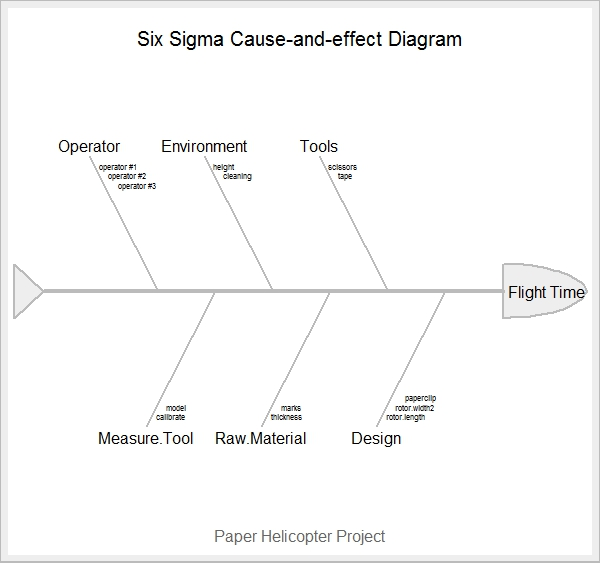
\includegraphics[width=0.7\linewidth]{./Rplot03}
\caption{}
\label{fig:Rplot03}
\end{figure}
\newpage
%----------------------------------------------------------------------------------------------%
\section{Data Set - \texttt{ss.data.ca} }
This data set is the volume measured in 20 bottles for a filling process in a winery
\begin{framed}
\begin{verbatim}
ss.data.ca
\end{verbatim}
\end{framed}

\begin{verbatim}
> ss.data.ca
   Volume
1  755.81
2  750.54
........
........
19 750.26
20 751.29
\end{verbatim}
\begin{figure}[h!]
\centering
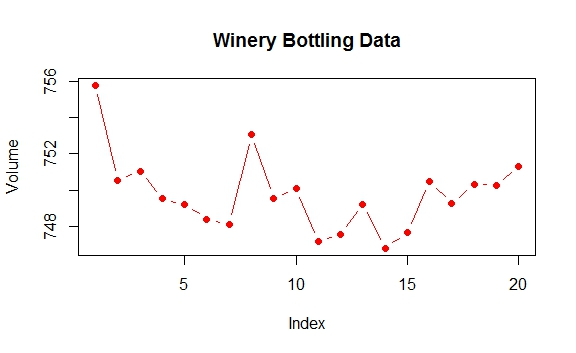
\includegraphics[width=0.9\linewidth]{./Winery}
\caption{}
\label{fig:Winery}
\end{figure}

%----------------------------------------------------------------------------------------------%
\newpage
\section{\texttt{ss.ca.z} Capability Indices}

Compute the Capability Indices of a process, Z (Sigma Score), $C_p$ and $C_{pk}$.
\begin{verbatim}
> ss.ca.cp(ss.data.ca$Volume,740, 760)
[1] 1.584136
> ss.ca.cpk(ss.data.ca$Volume,740, 760)
[1] 1.546513
> ss.ca.z(ss.data.ca$Volume,740,760)
[1] 3.139539
\end{verbatim}



\newpage
\section{Constructing Process Maps}
\begin{framed}
\begin{verbatim}
inputs.overall<-c("operators", "tools", "raw material", "facilities")
outputs.overall<-c("helicopter")
steps<-c("INSPECTION", "ASSEMBLY", "TEST", "LABELING")
\end{verbatim}
\end{framed}

\begin{framed}
\begin{verbatim}
#Inputs of process "i" are inputs of process "i+1"
input.output<-vector(mode="list",length=length(steps))
input.output[1]<-list(c("sheets", "..."))
input.output[2]<-list(c("sheets"))
input.output[3]<-list(c("helicopter"))
input.output[4]<-list(c("helicopter"))
\end{verbatim}
\end{framed}
Parameters of each process
\begin{framed}
\begin{verbatim}

x.parameters<-vector(mode="list",length=length(steps))

x.parameters[1]<-list(c(list(c("width", "NC")),list(c("operator", "C")),
                        list(c("Measure pattern", "P")), list(c("discard", "P"))))
x.parameters[2]<-list(c(list(c("operator", "C")),list(c("cut", "P")),
                        list(c("fix", "P")), list(c("rotor.width", "C")),
                        list(c("rotor.length",                                                                                "C")), 
                                                                                list(c("paperclip", "C")), list(c("tape", "C"))))
x.parameters[3]<-list(c(list(c("operator", "C")),
list(c("throw", "P")),
                        list(c("discard", "P")), 
                        list(c("environment", "N"))))
x.parameters[4]<-list(c(list(c("operator", "C")),
list(c("label", "P"))))
x.parameters

\end{verbatim}
\end{framed}

\begin{framed}
\begin{verbatim}
#Features of each process
y.features<-vector(mode="list",length=length(steps))
y.features[1]<-list(c(list(c("ok", "Cr"))))
y.features[2]<-list(c(list(c("weight", "Cr"))))
y.features[3]<-list(c(list(c("time", "Cr"))))
y.features[4]<-list(c(list(c("label", "Cr"))))
y.features
ss.pMap(steps, inputs.overall, outputs.overall,
        input.output, x.parameters, y.features,
        sub="Paper Helicopter Project")
\end{verbatim}
\end{framed}
\begin{figure}[h!]
\centering
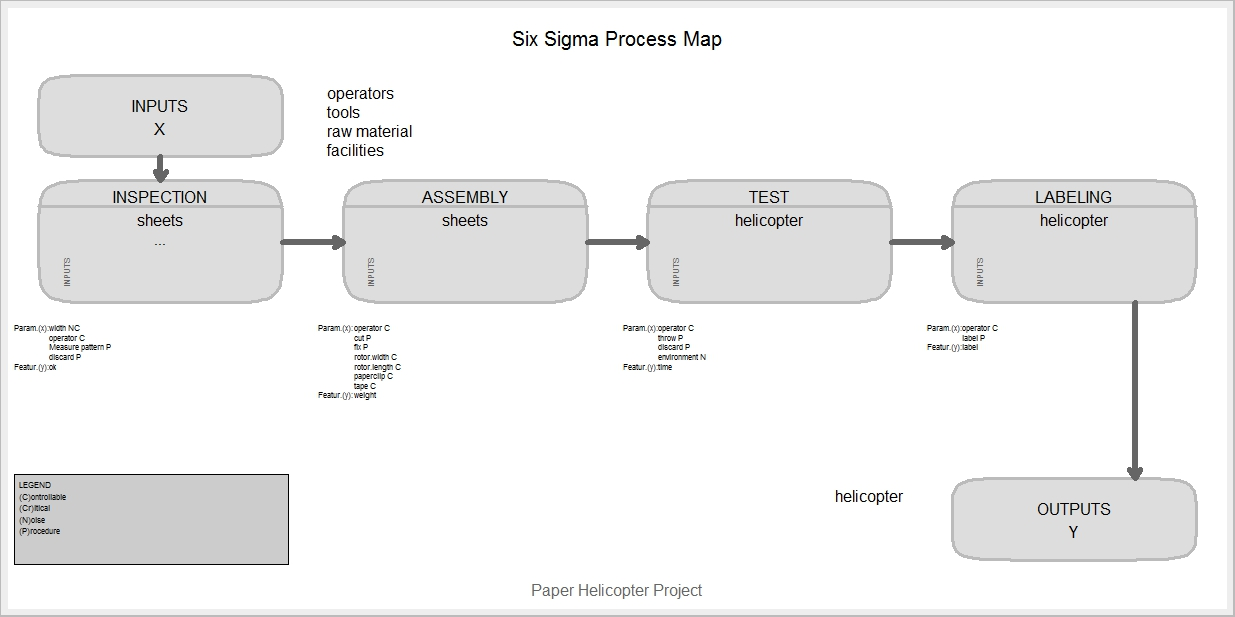
\includegraphics[width=0.9\linewidth]{./SixSigmaProcessMap}
\caption{}
\label{fig:SixSigmaProcessMap}
\end{figure}
%--------------------------------------------------- %
\newpage
\section{Loss Fucntion Aanalysis}
The Taguchi Loss Function is graphical depiction of loss developed by the Japanese business statistician Genichi Taguchi to describe a phenomenon affecting the value of products produced by a company. Praised by Dr. W. Edwards Deming (the business guru of the 1980s American quality movement),[1] it made clear the concept that quality does not suddenly plummet when, for instance, a machinist exceeds a rigid blueprint tolerance. Instead "loss" in value progressively increases as variation increases from the intended condition. This was considered a breakthrough in describing quality, and helped fuel the continuous improvement movement that since has become known as lean manufacturing.

\begin{figure}[h!]
\centering
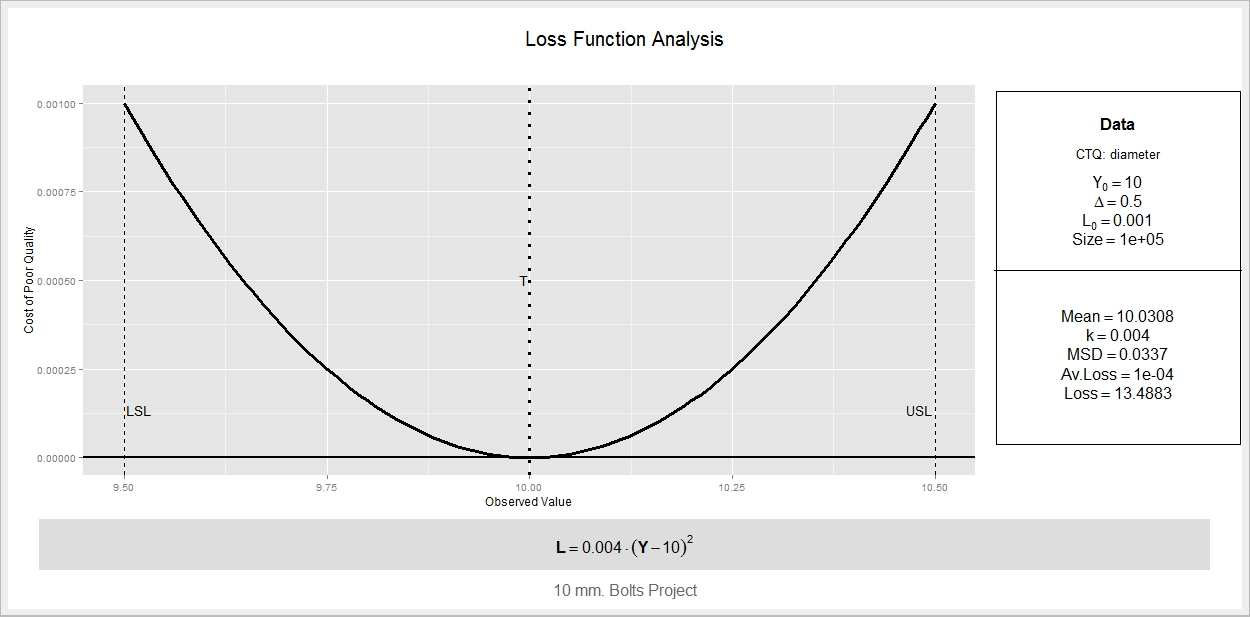
\includegraphics[width=0.7\linewidth]{./LossFunctionAnalysis}
\caption{}
\label{fig:LossFunctionAnalysis}
\end{figure}

\end{document}